% Options for packages loaded elsewhere
\PassOptionsToPackage{unicode}{hyperref}
\PassOptionsToPackage{hyphens}{url}
%
\documentclass[
  ignorenonframetext,
]{beamer}
\usepackage{pgfpages}
\setbeamertemplate{caption}[numbered]
\setbeamertemplate{caption label separator}{: }
\setbeamercolor{caption name}{fg=normal text.fg}
\beamertemplatenavigationsymbolsempty
% Prevent slide breaks in the middle of a paragraph
\widowpenalties 1 10000
\raggedbottom
\setbeamertemplate{part page}{
  \centering
  \begin{beamercolorbox}[sep=16pt,center]{part title}
    \usebeamerfont{part title}\insertpart\par
  \end{beamercolorbox}
}
\setbeamertemplate{section page}{
  \centering
  \begin{beamercolorbox}[sep=12pt,center]{part title}
    \usebeamerfont{section title}\insertsection\par
  \end{beamercolorbox}
}
\setbeamertemplate{subsection page}{
  \centering
  \begin{beamercolorbox}[sep=8pt,center]{part title}
    \usebeamerfont{subsection title}\insertsubsection\par
  \end{beamercolorbox}
}
\AtBeginPart{
  \frame{\partpage}
}
\AtBeginSection{
  \ifbibliography
  \else
    \frame{\sectionpage}
  \fi
}
\AtBeginSubsection{
  \frame{\subsectionpage}
}
\usepackage{lmodern}
\usepackage{amssymb,amsmath}
\usepackage{ifxetex,ifluatex}
\ifnum 0\ifxetex 1\fi\ifluatex 1\fi=0 % if pdftex
  \usepackage[T1]{fontenc}
  \usepackage[utf8]{inputenc}
  \usepackage{textcomp} % provide euro and other symbols
\else % if luatex or xetex
  \usepackage{unicode-math}
  \defaultfontfeatures{Scale=MatchLowercase}
  \defaultfontfeatures[\rmfamily]{Ligatures=TeX,Scale=1}
\fi
% Use upquote if available, for straight quotes in verbatim environments
\IfFileExists{upquote.sty}{\usepackage{upquote}}{}
\IfFileExists{microtype.sty}{% use microtype if available
  \usepackage[]{microtype}
  \UseMicrotypeSet[protrusion]{basicmath} % disable protrusion for tt fonts
}{}
\makeatletter
\@ifundefined{KOMAClassName}{% if non-KOMA class
  \IfFileExists{parskip.sty}{%
    \usepackage{parskip}
  }{% else
    \setlength{\parindent}{0pt}
    \setlength{\parskip}{6pt plus 2pt minus 1pt}}
}{% if KOMA class
  \KOMAoptions{parskip=half}}
\makeatother
\usepackage{xcolor}
\IfFileExists{xurl.sty}{\usepackage{xurl}}{} % add URL line breaks if available
\IfFileExists{bookmark.sty}{\usepackage{bookmark}}{\usepackage{hyperref}}
\hypersetup{
  pdftitle={305 Lecture 06 - Recursive Composition Rules},
  pdfauthor={Brian Weatherson},
  hidelinks,
  pdfcreator={LaTeX via pandoc}}
\urlstyle{same} % disable monospaced font for URLs
\newif\ifbibliography
\usepackage{graphicx,grffile}
\makeatletter
\def\maxwidth{\ifdim\Gin@nat@width>\linewidth\linewidth\else\Gin@nat@width\fi}
\def\maxheight{\ifdim\Gin@nat@height>\textheight\textheight\else\Gin@nat@height\fi}
\makeatother
% Scale images if necessary, so that they will not overflow the page
% margins by default, and it is still possible to overwrite the defaults
% using explicit options in \includegraphics[width, height, ...]{}
\setkeys{Gin}{width=\maxwidth,height=\maxheight,keepaspectratio}
% Set default figure placement to htbp
\makeatletter
\def\fps@figure{htbp}
\makeatother
\setlength{\emergencystretch}{3em} % prevent overfull lines
\providecommand{\tightlist}{%
  \setlength{\itemsep}{0pt}\setlength{\parskip}{0pt}}
\setcounter{secnumdepth}{-\maxdimen} % remove section numbering
\let\Tiny=\tiny

 \setbeamertemplate{navigation symbols}{} 

% \usetheme{Madrid}
 \usetheme[numbering=none, progressbar=foot]{metropolis}
 \usecolortheme{wolverine}
 \usepackage{color}
 \usepackage{MnSymbol}
% \usepackage{movie15}

\usepackage{amssymb}% http://ctan.org/pkg/amssymb
\usepackage{pifont}% http://ctan.org/pkg/pifont
\newcommand{\cmark}{\ding{51}}%
\newcommand{\xmark}{\ding{55}}%

\DeclareSymbolFont{symbolsC}{U}{txsyc}{m}{n}
\DeclareMathSymbol{\boxright}{\mathrel}{symbolsC}{128}
\DeclareMathAlphabet{\mathpzc}{OT1}{pzc}{m}{it}


% \usepackage{tikz-qtree}
% \usepackage{markdown}
% \usepackage{prooftrees}
% \forestset{not line numbering, close with = x}
% Allow for easy commas inside trees
\renewcommand{\,}{\text{, }}


\usepackage{tabulary}

\usepackage{open-logic-config}

\setlength{\parskip}{1ex plus 0.5ex minus 0.2ex}

\AtBeginSection[]
{
\begin{frame}
	\Huge{\color{darkblue} \insertsection}
\end{frame}
}

\renewenvironment*{quote}	
	{\list{}{\rightmargin   \leftmargin} \item } 	
	{\endlist }

\definecolor{darkgreen}{rgb}{0,0.7,0}
\definecolor{darkblue}{rgb}{0,0,0.8}

\newcommand{\starttab}{\begin{center}
\vspace{6pt}
\begin{tabular}}

\newcommand{\stoptab}{\end{tabular}
\vspace{6pt}
\end{center}
\noindent}


\newcommand{\sif}{\rightarrow}
\newcommand{\siff}{\leftrightarrow}
\newcommand{\EF}{\end{frame}}


\newcommand{\TreeStart}[1]{
%\end{frame}
\begin{frame}
\begin{center}
\begin{tikzpicture}[scale=#1]
\tikzset{every tree node/.style={align=center,anchor=north}}
%\Tree
}

\newcommand{\TreeEnd}{
\end{tikzpicture}
%\end{center}
}

\newcommand{\DisplayArg}[2]{
\begin{enumerate}
{#1}
\end{enumerate}
\vspace{-6pt}
\hrulefill

%\hspace{14pt} #2
%{\addtolength{\leftskip}{14pt} #2}
\begin{quote}
{\normalfont #2}
\end{quote}
\vspace{12pt}
}

\newenvironment{ProofTree}[1][1]{
\begin{center}
\begin{tikzpicture}[scale=#1]
\tikzset{every tree node/.style={align=center,anchor=south}}
}
{
\end{tikzpicture}
\end{center}
}

\newcommand{\TreeFrame}[2]{
\begin{columns}[c]
\column{0.5\textwidth}
\begin{center}
\begin{prooftree}{}
#1
\end{prooftree}
\end{center}
\column{0.45\textwidth}
%\begin{markdown}
#2
%\end{markdown}
\end{columns}
}

\newcommand{\ScaledTreeFrame}[3]{
\begin{columns}[c]
\column{0.5\textwidth}
\begin{center}
\scalebox{#1}{
\begin{prooftree}{}
#2
\end{prooftree}
}
\end{center}
\column{0.45\textwidth}
%\begin{markdown}
#3
%\end{markdown}
\end{columns}
}

\usepackage[bb=boondox]{mathalfa}
\DeclareMathAlphabet{\mathbx}{U}{BOONDOX-ds}{m}{n}
\SetMathAlphabet{\mathbx}{bold}{U}{BOONDOX-ds}{b}{n}
\DeclareMathAlphabet{\mathbbx} {U}{BOONDOX-ds}{b}{n}

\RequirePackage{bussproofs}
\RequirePackage[tableaux]{prooftrees}

\newenvironment{oltableau}{\center\tableau{}} %wff format={anchor = base west}}}
       {\endtableau\endcenter}
       
\newcommand{\formula}[1]{$#1$}

\usepackage{tabulary}
\usepackage{booktabs}

\def\begincols{\begin{columns}}
\def\begincol{\begin{column}}
\def\endcol{\end{column}}
\def\endcols{\end{columns}}

\usepackage[italic]{mathastext}
\usepackage{nicefrac}

\definecolor{mygreen}{RGB}{0, 100, 0}
\definecolor{mypink2}{RGB}{219, 48, 122}
\definecolor{dodgerblue}{RGB}{30,144,255}

\def\True{\textcolor{dodgerblue}{\text{T}}}
\def\False{\textcolor{red}{\text{F}}}

\title{305 Lecture 06 - Recursive Composition Rules}
\author{Brian Weatherson}
\date{July 6, 2020}

\begin{document}
\frame{\titlepage}

\begin{frame}{Plan for This Lecture}
\protect\hypertarget{plan-for-this-lecture}{}

\begin{itemize}
\tightlist
\item
  We're going to look at how and why we can iterate the translation
  procedures we've been investigating.
\end{itemize}

\end{frame}

\begin{frame}{Recursion}
\protect\hypertarget{recursion}{}

The language of propositional logic has some fairly simple composition
rules.

\begin{itemize}
\tightlist
\item
  It says what the basic sentences are.
\item
  It has some rules saying that if some things are sentences, so are
  some other things.
\end{itemize}

The effect is that there are an infinity of possible sentences.

\end{frame}

\begin{frame}{Natural Language Recursion}
\protect\hypertarget{natural-language-recursion}{}

As speakers of a human language, you're used to this kind of recursion.
All of these are sentences.

\begin{itemize}[<+->]
\tightlist
\item
  It will rain.
\item
  Alex thinks that it will rain.
\item
  Kim thinks that Alex thinks that it will rain.
\item
  Alex thinks that Kim thinks that Alex thinks that it will rain.
\item
  And so on, to infinity, without adding any more words.
\end{itemize}

\end{frame}

\begin{frame}{Recursive Rule}
\protect\hypertarget{recursive-rule}{}

\begin{itemize}
\tightlist
\item
  If \emph{S} is a sentence, and \emph{N} is a name, then \emph{N thinks
  that S} is a sentence.
\item
  Note that the output of this rule can be the inpute to a new instance
  of it.
\end{itemize}

\end{frame}

\begin{frame}{Formal Language Recursion}
\protect\hypertarget{formal-language-recursion}{}

\begin{itemize}
\tightlist
\item
  The letters \(P, Q, R...\) are sentences.
\item
  If \emph{S} and \emph{T} are sentences, then so are:
\end{itemize}

\begin{enumerate}
\tightlist
\item
  \(\neg S\)
\item
  \(S \vee T\)
\item
  \(S \wedge T\)
\item
  \(S \rightarrow T\)
\item
  \(S \leftrightarrow T\)
\end{enumerate}

\end{frame}

\begin{frame}{Multiple Steps}
\protect\hypertarget{multiple-steps}{}

So these are all sentences. (Note that I'm playing fast and loose with
parentheses here.)

\begin{enumerate}
\tightlist
\item
  \(P\)
\item
  \(Q\)
\item
  \(P \wedge Q\)
\item
  \(Q \rightarrow (P \wedge Q)\)
\item
  \(\neg P\)
\item
  \(Q \vee \neg P\)
\item
  \((Q \rightarrow (P \wedge Q)) \leftrightarrow (Q \vee \neg P)\)
\end{enumerate}

The last one follows from the fact that 4 and 6 are sentences.

\end{frame}

\begin{frame}{Main Connective}
\protect\hypertarget{main-connective}{}

For any sentence you can make, there will be a `last step' in the
demonstration that it is a sentence.

\begin{itemize}
\tightlist
\item
  That last step will involve copying down 1 or 2 other sentences, and
  adding a connective.
\item
  On the previous slide, you copy down 4 and 6, and put a
  \(\leftrightarrow\) between them.
\item
  That connective you add is the \textbf{main connective} of the
  sentence.
\item
  It covers all the material in the sentence.
\end{itemize}

\end{frame}

\begin{frame}{Main Connective}
\protect\hypertarget{main-connective-1}{}

A binary connective is the main connective if (and only if) either side
of it are two complete sentences.

\begin{quote}
\(P \wedge (Q \rightarrow R)\)
\end{quote}

The \(\wedge\) is the main connective because either side of it are

\begin{itemize}
\tightlist
\item
  \(P\)
\item
  \((Q \rightarrow R)\)
\end{itemize}

And they are both sentences.

\end{frame}

\begin{frame}{Main Connective}
\protect\hypertarget{main-connective-2}{}

A binary connective is the main connective if (and only if) either side
of it are two complete sentences.

\begin{quote}
\(P \wedge (Q \rightarrow R)\)
\end{quote}

The \(\rightarrow\) is the main connective because either side of it are

\begin{itemize}
\tightlist
\item
  \(P \wedge (Q\)
\item
  \(R)\)
\end{itemize}

And they are not both sentences.

\end{frame}

\begin{frame}{A Worked Example}
\protect\hypertarget{a-worked-example}{}

\begin{figure}
\centering
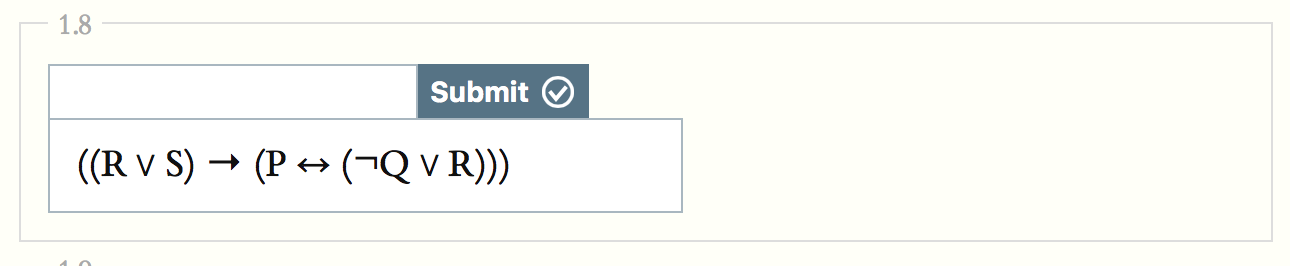
\includegraphics{../images/class02/1.png}
\caption{Step 1}
\end{figure}

\end{frame}

\begin{frame}{A Worked Example}
\protect\hypertarget{a-worked-example-1}{}

\begin{figure}
\centering
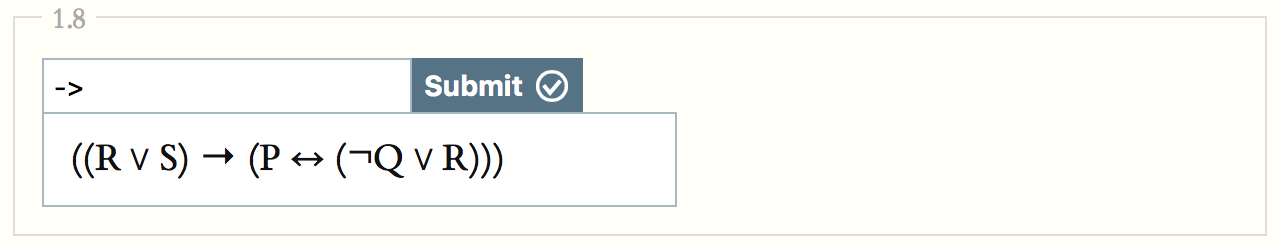
\includegraphics{../images/class02/2.png}
\caption{Step 2}
\end{figure}

\end{frame}

\begin{frame}{A Worked Example}
\protect\hypertarget{a-worked-example-2}{}

\begin{figure}
\centering
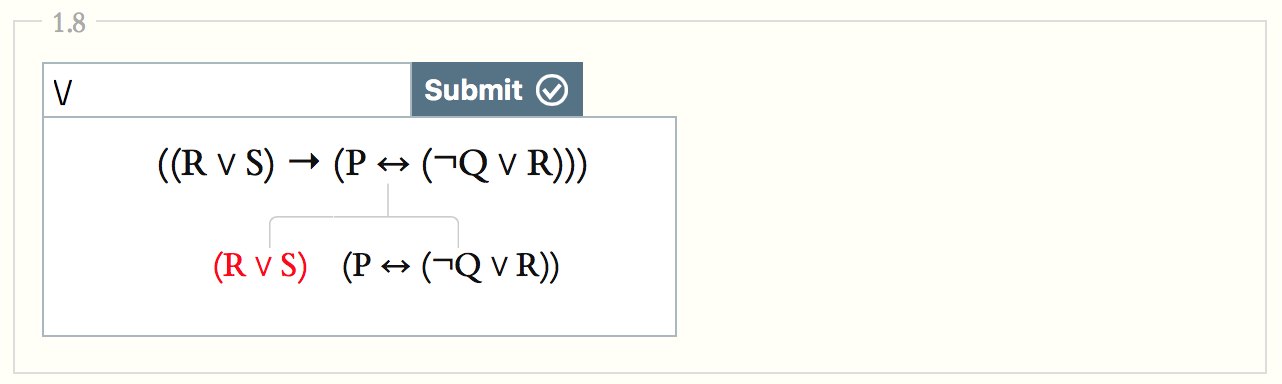
\includegraphics{../images/class02/3.png}
\caption{Step 3}
\end{figure}

\end{frame}

\begin{frame}{A Worked Example}
\protect\hypertarget{a-worked-example-3}{}

\begin{figure}
\centering
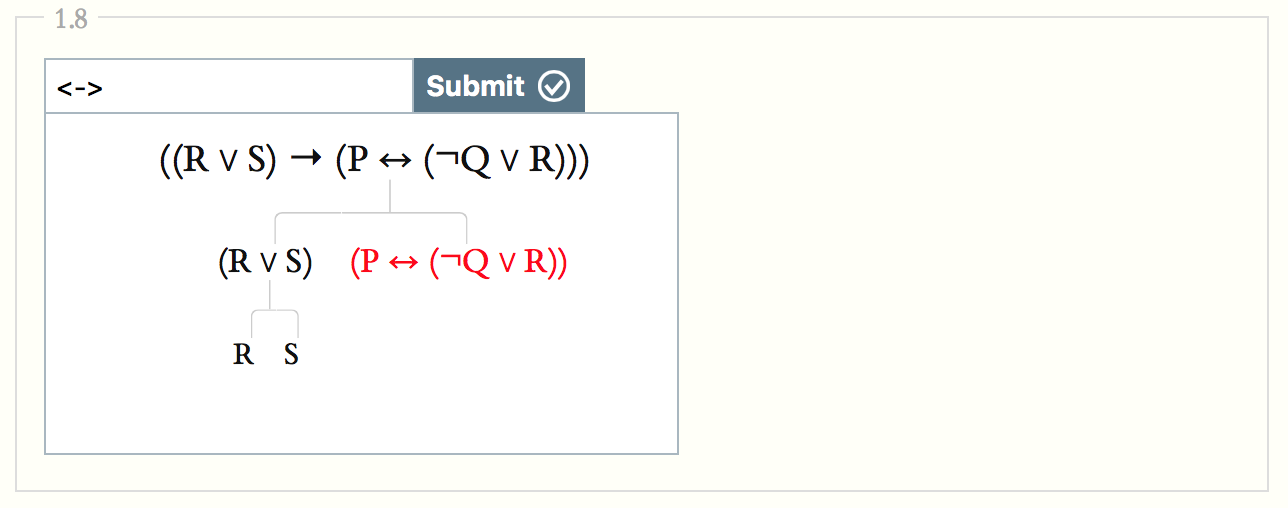
\includegraphics{../images/class02/4.png}
\caption{Step 4}
\end{figure}

\end{frame}

\begin{frame}{A Worked Example}
\protect\hypertarget{a-worked-example-4}{}

\begin{figure}
\centering
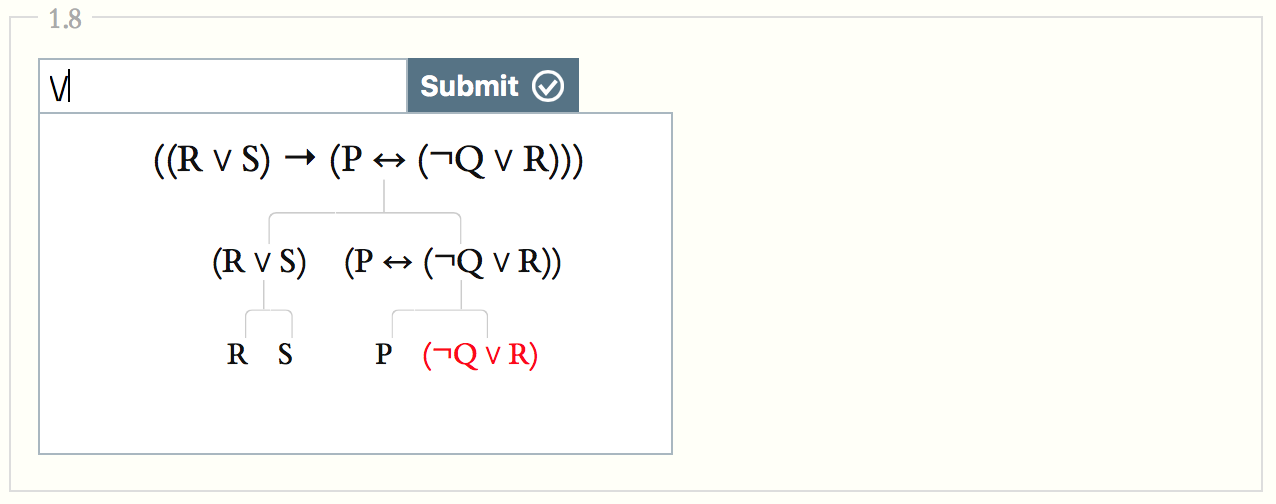
\includegraphics{../images/class02/5.png}
\caption{Step 5}
\end{figure}

\end{frame}

\begin{frame}{A Worked Example}
\protect\hypertarget{a-worked-example-5}{}

\begin{figure}
\centering
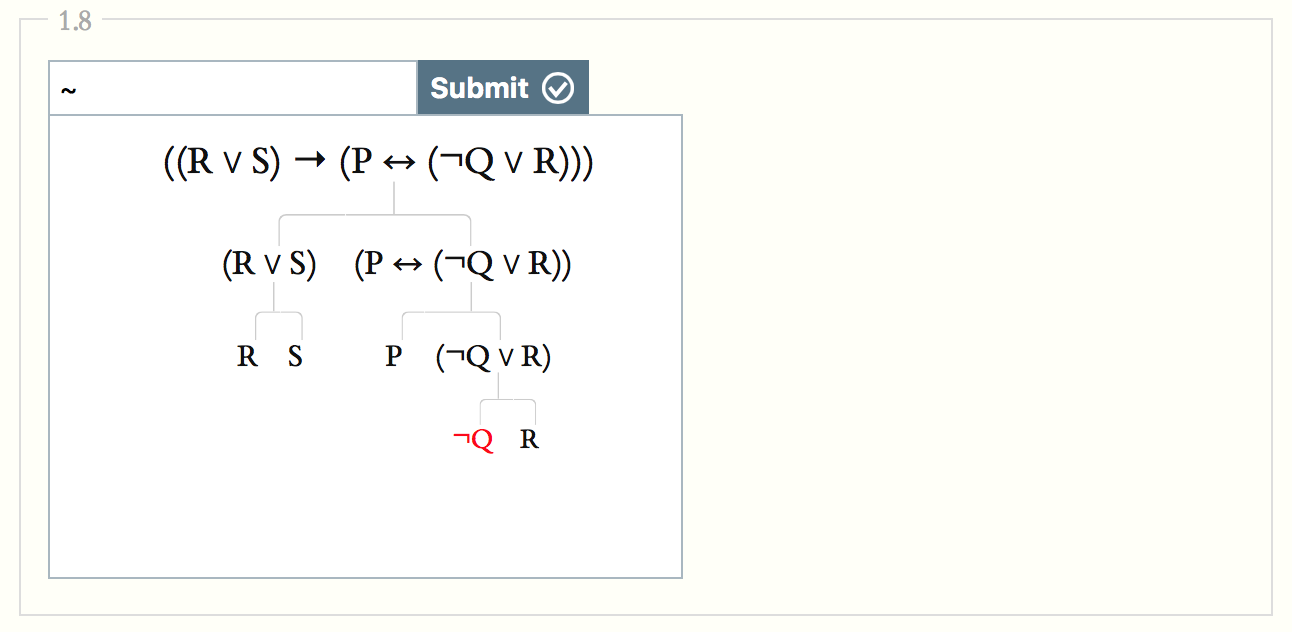
\includegraphics{../images/class02/6.png}
\caption{Step 6}
\end{figure}

\end{frame}

\begin{frame}{For Next Time}
\protect\hypertarget{for-next-time}{}

\begin{itemize}
\tightlist
\item
  That's all for today's lectures
\item
  For next time, read Chapter 3 of The Carnap Book
\item
  We're going to start applying these tools to analysing arguments.
\end{itemize}

\end{frame}

\end{document}
